\documentclass{standalone}

\usepackage{tikz}

\newcommand{\tree}{
\draw[line cap=round] (0,0) -- (-1,-1);
\draw[line cap=round] (0,0) -- ( 0,-1);
\draw[line cap=round] (0,0) -- ( 1,-1);
\fill[black] (-1,-1) -- (-1.1,-1.25) -- (-0.9,-1.25) -- cycle;
\draw[]      (0,-1) -- (-1.1+1,-1.25) -- (-0.9+1,-1.25) -- cycle;
}

\begin{document}
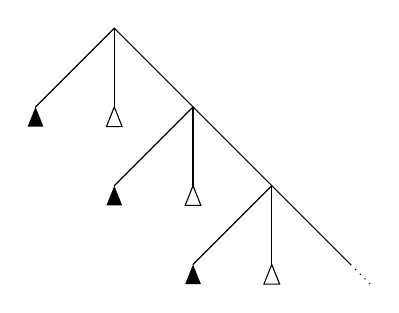
\begin{tikzpicture}
  
  \tree
  \begin{scope}[shift={(1,-1)}] \tree
  \begin{scope}[shift={(1,-1)}] \tree
  \begin{scope}[shift={(1,-1)}]
    \draw[dotted] (0,0) -- (0.25,-0.25);
  \end{scope}
  \end{scope}
  \end{scope}
  
\end{tikzpicture}
\end{document}